\chapter{Case Studies}

%do the usual introduction
% then explain wtf the idea is
\section{Scenario 1: Demand-Response Misinformation Campaign}
\label{demandresponsesection}
%First: Explain throuhout the scenario
%Then define assumptions
%Then define parameters
%Then simulation results
%This Scenario should also be the one with the total framework

With the increased usage of information and communication 
technologies (ICT), new methods of influencing
consumer demand patterns are possible. 
These can be used by electrical companies to change the 
demand curve over time, ideally to reduce peak loads 
and thus increasing the efficiency of the electrical grid.
A realistic power demand, as shown in Figure \ref{duckcurve}, tend 
to vary greatly during the day. This leads to inefficiency,
since excess supply sources need to be build to satisfy customers
during peak hours. The idea is to lead consumers to shift
their consumption from peak demand hours to low demand hours,
thus reducing the variation of demand over time and allowing
for more efficient management of the power grid infrastructure.
This concept of changing the demand to match the 
available supply of electricity is called demand-response. 
One method to influence the consumer demand is by real time 
pricing (RTP). With RTP, the electricity prices change
dynamically based on the total electricity demand.
The price changes are then forwarded to the customers with ICTs, 
who are thus informed of the price changes.
The idea of RTP is that consumers change their electricity demand
by shifting activities with a high electricity usage, 
such as washing clothes or cooking, to time periods 
where the total electricity demand and thus the prices
are lower. This leads to reduced peak energy consumption. 
RTP was already used in a variety of programs
under real life conditions \cite{barbose2004survey}.
Studies showed the benefits of such programs \cite{albadi2008summary}.

\begin{figure}[!ht]
    \center
    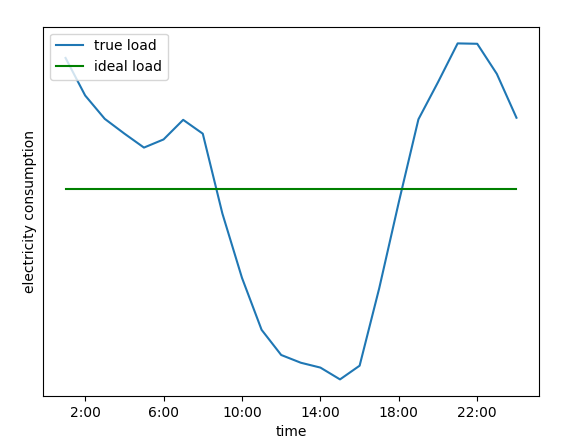
\includegraphics[scale=.75]{figs/duckcurve.png}
    \caption{real power load and the ideal power load for the 
    power grid infrastructure}
    \label{duckcurve}
\end{figure}

Problematic is if a false pricing rumor spreads through social media.
In 2022, changes in the verification policies of Twitter lead to users being able 
to impersonate well-known brands such as Pepsi, leading to Twitter 
users being unable to determine which social media channels were
posting trustworthy information \cite{twitterchaos}. One user could
have used the policy changes of Twitter to impersonate 	utility companies
and to advertise a false reduction of energy prices, leading to customers
believing the information and increasing their energy consumption as a 
reaction. Another possibility would be that hackers would force access to the
social media profiles of 	utility companies and start sending false 
information to its customers. Hackers were already able to gain access
to the social media profiles of multinational companies in the past
\cite{twitterhacker}. Hackers could also spread misinformation in regards
to a false reduction in prices, thus leading to changing consumer demand.

% HERE AN EXAMPLE TWITTER POST

Based on the information, a possible scenario could be that hackers would
access the social media profiles of a well-known utility company
to spread the information that the energy prices would be reduced by 
a signifiant factor at a specific time. This information would then be 
spread around social media, reaching many customers of the company.


\section{Scenario 2: Coordinated Action of Extremists 
against the Electrical Grid}

Echo chambers on various social media websites allow people to 
hear biased opinions and news which confirm their views on 
various topics \cite{terren2021echo}. This leads to political
polarization and extremism \cite{van2022banality}.
These people in turn can try to fight the established political
system. Research shows that social media influence people
to commit hate crimes \cite{muller2021fanning}.
In general, the number of violent incidents caused by
extremists, specially right-wing extremists, is rising 
\cite{koehler2016right}. 
Most of the criminal acts caused by political extremism 
in germany are in the fields of property damage, 
propaganda crimes, insults and hate speech \cite{bmicrimestatistics}.
But extremists also cause more serious crimes. In 2022,
right-wing extremists planned to sabotage the electrical grid 
infrastructure by destroying power lines \cite{anschlagstrom}.
Thus, it can be seen that critical infrastructure may also be a target
for political extremists. 

Another way to target critical infrastructure is with a coordinated
actions which in its sum can damage the infrastructure. The 
reasons for a group of people to take such action may be harmless,
such as the Earth day, where people where encouraged to switch off their 
lights and appliances to save energy \cite{earthday}.
But extremists could also synchronize their actions to reduce their
power consumption to a minimum, thus mismatching electricity supply
and demand by a considerable degree. Electricity companies would 
then need to deal with a sudden surplus of electricity.

Given the previous information, a possible scenario could be 
that extremists plan to turn off all their electrical devices at 
a specific time to destabilize the electrical infrastructure. The
time would be announced in advance.


\section{Scenario 3: Mass Evacuation of a City due to a Disaster}

Sometimes the conditions under a disaster get so extreme that 
authorities choose to order the evacuation of the affected population.
For these types of evacuation, the autorities may use emergency channels 
to inform the population of the evacuation.
But people may also choose to leave the city in masses on their own accord.
The information of a possible disaster, such as a wildfire, reaching the
city soon or other disasters such as a widespread terrorist attacks 
in the city.
If people decide to leave their homes to flee from the disaster, they 
will mostly use their cars as the mode of transportation.
In the future, the increased adoption of electric vehicles (EV)
may lead to people needing to recharge their EVs if they wish 
to drive them. An evacuation could lead to many people charging
their cars at the same time, thus creating excess demand that 
the infrastructure is unable to handle. 

Given the previous assumptions, a possible scenario could be that 
rumors about a wildfire spreading towards a city leads to people
trying to leave the city in masses. In addition, a significant 
amount of people drive EVs, thus giving them the need to charge
their cars before they are able to leave the city.


\section{Scenario 4: Mass Showering after a Chemical Accident}
%This Scenario should also be the one with the total framework

With the increasing usage of ICTs in the population, it allows for 
new methods to communicate with people about extreme circumstances
such as natural disasters or other catastrophes. In 2022,
a new warning system called Cell Broadcast was introduced in Germany
\cite{techrichtlinie}. Cell Broadcast can be used to warn the population
of emergencies by sending all cellphone users in the 
region of interest a message with a loud alert tone.

Germany has one of the biggest chemical industry sectors in the world.
It is home to big chemical factories in cities such as Ludwigshafen and
Darmstadt. Areas with chemical factories have the risk of being
victims of chemical accidents.

A possible scenario would be that a chemical accident in a 
factory near a major city would lead to dangerous chemicals 
leaking out. These chemicals would spread through the air 
and adhere to the skin of humans, leading to serious 
health problems if they stayed on the skin for too long.
Thus, the city's government would use Cell Broadcast to
instruct the population to close their windows and 
to take a shower to remove the chemicals from their bodies.
Therefore, most people would take showers at the same time.


% Questions: how to define the parameters
% For some, I can use a dataset and use this as an analogy
% But e.g. scenario 2 it doesnt work well
% how can I put thing out of my ass
% what could be interesting parameter tweakings 